\documentclass[10pt,aspectratio=169,serif]{beamer}

\usepackage[fontset=none, scheme=plain]{ctex}
\IfFontExistsTF{Songti SC}{%
	\setCJKmainfont{Songti SC}[AutoFakeSlant=0.2]%
	\setCJKsansfont{Songti SC}[AutoFakeSlant=0.2]%
}{%
	\setCJKmainfont{FandolSong-Regular}[Extension=.otf,BoldFont=FandolSong-Bold,AutoFakeSlant=0.2]%
	\setCJKsansfont{FandolSong-Regular}[Extension=.otf,BoldFont=FandolSong-Bold]%
}
\usepackage{amsmath,amssymb,graphicx,tikz,booktabs,multicol,calligra}
\usepackage{pgfplots}
\pgfplotsset{compat=1.18}
\usepackage{tcolorbox}
\tcbuselibrary{skins}
\usepackage{XyygU}
\usepackage{caption}
\captionsetup[figure]{name=图,labelsep=period}

\usetikzlibrary{arrows.meta,positioning,calc}

\setlength{\abovedisplayskip}{0pt plus 2pt minus 2pt}
\setlength{\belowdisplayskip}{0pt plus 2pt minus 2pt}

\title[5.6 $y=A\sin(\omega x+\varphi)$ 练习]{5.6 函数 $y=A\sin(\omega x+\varphi)$（练习）}
\subtitle{图象变换 \& 五点法作图}
\author{}
\institute{}
\date{2026-10-16}

\begin{document}

\begin{frame}
  \titlepage
\end{frame}

% --- 1 ---
\begin{frame}[t]{第1题：画一个周期内的简图}
\textbf{1.} 画出下列函数在长度为一个周期的闭区间上的简图，并用信息技术检验：
\begin{enumerate}
  \item $y=\dfrac12\sin x$；\qquad
  \item $y=\sin 3x$；
  \item $y=\sin\!\left(x-\dfrac{\pi}{3}\right)$；\qquad
  \item $y=2\sin\!\left(2x-\dfrac{\pi}{4}\right)$。
\end{enumerate}
\end{frame}

\begin{frame}[t]{第1题 解答：(1) $y=\frac12\sin x$}
\begin{tcolorbox}[colback=orange!10,colframe=orange,title=\textbf{解}]
振幅 $\frac12$，周期 $2\pi$，初相 $0$。由 $y=\sin x$ 图象上所有点的纵坐标缩短到原来的 $\frac12$（横坐标不变）得到。
\end{tcolorbox}
\begin{center}
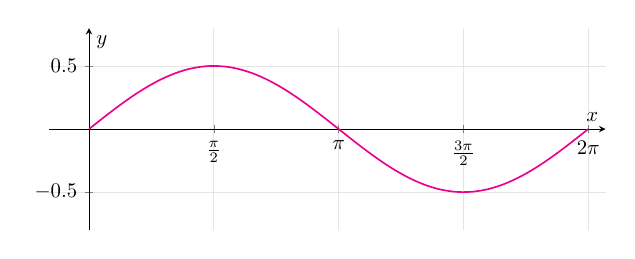
\begin{tikzpicture}[scale=0.75]
\begin{axis}[width=11cm,height=5cm,axis lines=middle,xlabel=$x$,ylabel=$y$,
xmin=-0.5,xmax=6.5,ymin=-0.8,ymax=0.8,
xtick={1.5708,3.1416,4.7124,6.2832},xticklabels={$\frac{\pi}{2}$,$\pi$,$\frac{3\pi}{2}$,$2\pi$},
ytick={-0.5,0.5},grid=major,grid style={gray!20}]
\addplot[thick,magenta,domain=0:6.2832,samples=100] {0.5*sin(deg(x))};
\end{axis}
\end{tikzpicture}
\end{center}
\end{frame}

\begin{frame}[t]{第1题 解答：(2) $y=\sin 3x$}
\begin{tcolorbox}[colback=orange!10,colframe=orange,title=\textbf{解}]
振幅 $1$，周期 $T=\dfrac{2\pi}{3}$。由 $y=\sin x$ 图象上所有点的横坐标缩短到原来的 $\frac13$（纵坐标不变）得到。
\end{tcolorbox}
\begin{center}
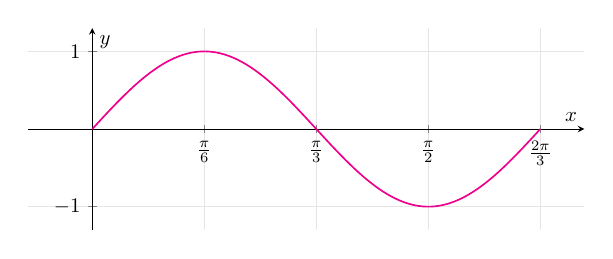
\begin{tikzpicture}[scale=0.75]
\begin{axis}[width=11cm,height=5cm,axis lines=middle,xlabel=$x$,ylabel=$y$,
xmin=-0.3,xmax=2.3,ymin=-1.3,ymax=1.3,
xtick={0.5236,1.0472,1.5708,2.0944},xticklabels={$\frac{\pi}{6}$,$\frac{\pi}{3}$,$\frac{\pi}{2}$,$\frac{2\pi}{3}$},
ytick={-1,1},grid=major,grid style={gray!20}]
\addplot[thick,magenta,domain=0:2.0944,samples=100] {sin(deg(3*x))};
\end{axis}
\end{tikzpicture}
\end{center}
\end{frame}

\begin{frame}[t]{第1题 解答：(3) $y=\sin(x-\frac{\pi}{3})$}
\begin{tcolorbox}[colback=orange!10,colframe=orange,title=\textbf{解}]
振幅 $1$，周期 $2\pi$，初相 $-\frac{\pi}{3}$。由 $y=\sin x$ 图象向右平移 $\frac{\pi}{3}$ 个单位长度得到。
\end{tcolorbox}
\begin{center}
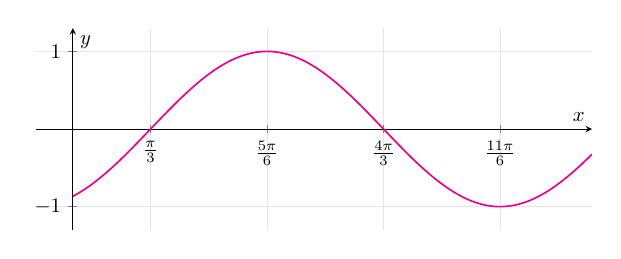
\begin{tikzpicture}[scale=0.75]
\begin{axis}[width=11cm,height=5cm,axis lines=middle,xlabel=$x$,ylabel=$y$,
xmin=-0.5,xmax=7,ymin=-1.3,ymax=1.3,
xtick={1.0472,2.618,4.1888,5.7596},xticklabels={$\frac{\pi}{3}$,$\frac{5\pi}{6}$,$\frac{4\pi}{3}$,$\frac{11\pi}{6}$},
ytick={-1,1},grid=major,grid style={gray!20}]
\addplot[thick,magenta,domain=0:7,samples=100] {sin(deg(x-pi/3))};
\end{axis}
\end{tikzpicture}
\end{center}
\end{frame}

\begin{frame}[t]{第1题 解答：(4) $y=2\sin(2x-\frac{\pi}{4})$}
\begin{tcolorbox}[colback=orange!10,colframe=orange,title=\textbf{解}]
振幅 $2$，周期 $T=\pi$，初相 $-\frac{\pi}{4}$，即 $2x-\frac{\pi}{4}=0$ 时 $x=\frac{\pi}{8}$。
\end{tcolorbox}
\begin{center}
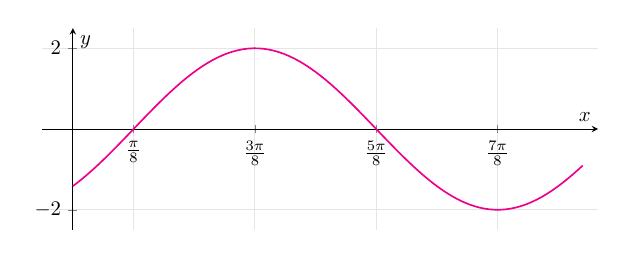
\begin{tikzpicture}[scale=0.75]
\begin{axis}[width=11cm,height=5cm,axis lines=middle,xlabel=$x$,ylabel=$y$,
xmin=-0.2,xmax=3.4,ymin=-2.5,ymax=2.5,
xtick={0.3927,1.1781,1.9635,2.7489},xticklabels={$\frac{\pi}{8}$,$\frac{3\pi}{8}$,$\frac{5\pi}{8}$,$\frac{7\pi}{8}$},
ytick={-2,2},grid=major,grid style={gray!20}]
\addplot[thick,magenta,domain=0:3.3,samples=100] {2*sin(deg(2*x-pi/4))};
\end{axis}
\end{tikzpicture}
\end{center}
\end{frame}

% --- 2 ---
\begin{frame}[t]{第2题：图象变换选择}
\textbf{2.} 已知函数 $y=3\sin\!\left(x+\dfrac{\pi}{5}\right)$ 的图象为 $C$。
\begin{enumerate}
  \item 为得到 $y=3\sin\!\left(x-\dfrac{\pi}{5}\right)$ 的图象，只要把 $C$ 上所有的点（\quad）。
  \item 为得到 $y=3\sin\!\left(2x+\dfrac{\pi}{5}\right)$ 的图象，只要把 $C$ 上所有的点（\quad）。
  \item 为得到 $y=4\sin\!\left(x+\dfrac{\pi}{5}\right)$ 的图象，只要把 $C$ 上所有的点（\quad）。
\end{enumerate}
\end{frame}

\begin{frame}[t]{第2题 解答}
\begin{tcolorbox}[colback=orange!10,colframe=orange,title=\textbf{解}]
(1) $x-\dfrac{\pi}{5}=\left(x-\dfrac{2\pi}{5}\right)+\dfrac{\pi}{5}$，即图象上所有点向右平移 $\dfrac{2\pi}{5}$ 个单位长度。\alert{选 (C)}。

(2) $3\sin(2x+\frac{\pi}{5})$ 与 $3\sin(x+\frac{\pi}{5})$ 相比，$\omega$ 由 $1$ 变为 $2$，周期缩短一半，即横坐标缩短到原来的 $\frac12$，纵坐标不变。\alert{选 (B)}。

(3) 振幅由 $3$ 变为 $4$，即纵坐标伸长到原来的 $\frac43$ 倍，横坐标不变。\alert{选 (C)}。
\end{tcolorbox}
\end{frame}

% --- 3 ---
\begin{frame}[t]{第3题：$y=\frac23\sin(\frac12 x-\frac{\pi}{4})$ 的变换}
\textbf{3.} 函数 $y=\dfrac23\sin\!\left(\dfrac12 x-\dfrac{\pi}{4}\right)$ 的图象与正弦曲线有什么关系？
\end{frame}

\begin{frame}[t]{第3题 解答}
\begin{tcolorbox}[colback=orange!10,colframe=orange,title=\textbf{解}]
由 $y=\sin x$ 图象经过以下变换得到：
\begin{enumerate}
  \item 向右平移 $\dfrac{\pi}{4}$ 个单位长度，得 $y=\sin\!\left(x-\dfrac{\pi}{4}\right)$；
  \item 横坐标伸长到原来的 $2$ 倍（纵坐标不变），得 $y=\sin\!\left(\dfrac12 x-\dfrac{\pi}{4}\right)$；
  \item 纵坐标缩短到原来的 $\dfrac23$（横坐标不变），即得所求。
\end{enumerate}
振幅 $\dfrac23$，周期 $T=4\pi$，初相 $-\dfrac{\pi}{4}$。
\end{tcolorbox}
\begin{center}
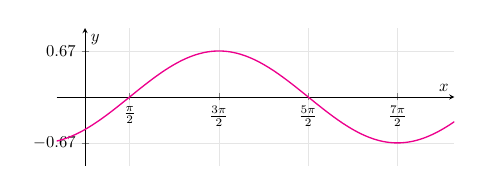
\begin{tikzpicture}[scale=0.6]
\begin{axis}[width=10cm,height=4.5cm,axis lines=middle,xlabel=$x$,ylabel=$y$,
xmin=-1,xmax=13,ymin=-1,ymax=1,xtick={1.57,4.71,7.85,11},xticklabels={$\frac{\pi}{2}$,$\frac{3\pi}{2}$,$\frac{5\pi}{2}$,$\frac{7\pi}{2}$},
ytick={-0.667,0.667},grid=major,grid style={gray!20}]
\addplot[thick,magenta,domain=-1:13,samples=200] {0.6667*sin(deg(0.5*x-pi/4))};
\end{axis}
\end{tikzpicture}
\end{center}
\end{frame}

% --- 4 ---
\begin{frame}[t]{第4题：$y=\sin(x+\frac{\pi}{12}),\ x\in[0,+\infty)$}
\textbf{4.} 函数 $y=\sin\!\left(x+\dfrac{\pi}{12}\right)$，$x\in\left[0,+\infty\right)$ 的图象与正弦曲线有什么关系？
\end{frame}

\begin{frame}[t]{第4题 解答}
\begin{tcolorbox}[colback=orange!10,colframe=orange,title=\textbf{解}]
形状与 $y=\sin x$ 完全相同：振幅 $1$，周期 $2\pi$。
\begin{enumerate}
  \item 由 $y=\sin x$ 图象向左平移 $\dfrac{\pi}{12}$ 个单位长度，得到 $y=\sin\!\left(x+\dfrac{\pi}{12}\right)$ 的完整图象；
  \item 再取 $x\ge 0$ 的部分，即得所求函数图象。它不再是完整的周期曲线，而是从 $x=0$ 开始、向右无限延伸的一段（起点处 $y=\sin\dfrac{\pi}{12}$）。
\end{enumerate}
\end{tcolorbox}
\end{frame}

\begin{frame}[c]
  \begin{center}
    {\Huge\calligra Thanks!}
  \end{center}
\end{frame}

\end{document}
